\subsection{Controller}
Der Infineon XMC 1xxx48 gehört zu der Familie der ARM Cortex -M0 Prozessoren und ist ein 32-bit Industrial Microcontroller und wird mit 48~MHz externer Clock betrieben. Die 48 im Namen des Prozessors steht für die Anzahl der Pins. Der interne Timer läuft mit 96Mhz. Unteranderem besitzt die CCU4 von dem Prozessor 2x4 16 bit Timer. Außerdem bietet der XMC einen 12 bit A/D Wandler, welcher für die Analogmessung eine viel genauere Auflösung bieten kann als ein 8 bit A/D Wandler. Die Betriebsspannung des Prozessors beträgt 3,3~V. Die Auswahl des Controller wurde getroffen, weil der standardmäßig auch schon bei Tinkerforge eingsetz wird und uns für den Prototypen vorgeben wurde. Der Controller bietet eine weitere Besonderheit beim Programmieren, siehe dazu das Unterkapitel \ref{Besonderheit der Software}\\


\subsection{Sender}%Bearbeiten
Um eine Trennung zwischen der CPU (3,3~V) und dem Hochsetzsteller (5~V-20~V), dessen Aufgabe es ist eine höhere Spannung an der Ultraschallkapsel zur erzeugen, zu ermöglichen, wurde ein weiteres Bauteil benötigt. Dafür wurde das IC A5950 (Voll Brücke) ausgewählt.
Die H-Brücke kann eine angeschlossene Last mit der vom Hochsetzstellers erzeugten Spannung versorgen. Deren Frequenz wird über das Signal an dem Anschluss Phase von der CPU vorgegeben. An Out1 und Out2 wird das Ausgangssignal abgegriffen. Für die genaue Beschaltung des ICs siehe Anhang Datenblatt “Schimatic A5950“.


\subsection{Hochsetzsteller}%Dannat

Tinkerforge nutzt schon eine Variante eines Hochsetzstellers auf ihren Platinen somit konnte der Aufbau und die Bauteilauswahl nur auf die Variable Ausgangspannungs erweitert werden. Die Standardschaltung, von Tinkerforge, wurde an dem Eingang der Feedbackspannung mit einem Potentiometer (RV1) erweitert, um die gewünschte Variable Spannung zubekommen.\\
Die Ausgangsspannung wird mit den externen Widerständen RV1, R13 und R2 eingestellt (siehe Grund Schaltung Datenblatt S.11). Ein Wert von ca. \(\displaystyle 13,3~K\Omega \) wurde für R2 empfohlen. Mit den Potentiometer (RV1) lässt sich die Ausgangsspannung bei 5~V Eingangsspannung bis 21,5~V einstellen. In der Formel werden die Widerstände RV1 und R13 zum Ersatz widerstand(Re) zusammengefasst.
\onehalfspacing \\
\(\displaystyle Re=R2*\left(\frac{Vout}{1,23}-1\right) \Rightarrow Vout=\left(\frac{Re}{R2}+1\right)*1,23\) 
\singlespacing
\begin{center}
\begin{minipage}{0.75\textwidth}
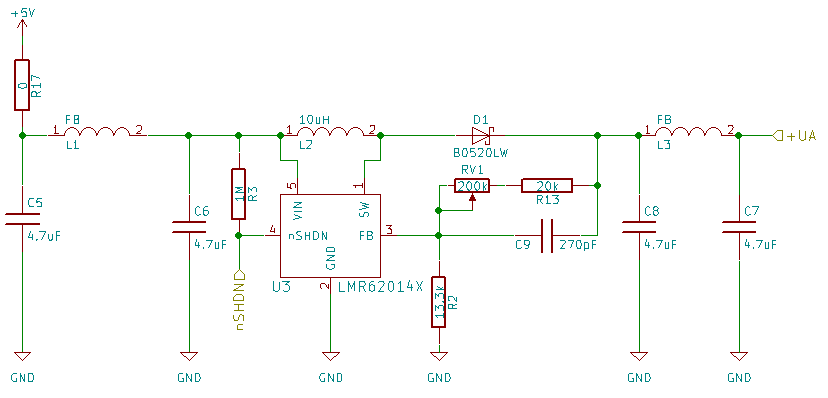
\includegraphics[width=1\textwidth%, draft
]{Abbildungen/Pumpe.png}
\captionof{figure}{Hochsetzsteller}
\label{fig:Hochsetzsteller}
\end{minipage}\\
\end{center}

\subsection{Ultraschallkapsel}%bearbeiten
Für den Prototypen wurden mehrere Kapseln vereschiedener Hersteller bestellt. Dieses geschah um Unterschiede der verschiedenpreisigen Bauteile zu ermitteln und festzustellen, welches Preissegment die nötige Qualität für die vorliegende Anwendung erfüllt.


\subsection{Filter}%bearbeiten
Die Filterschaltung wurde mit einem Hochpassfilter (CR Glied) bestückt bestehend aus einem Kodensator (C12) und einem Widerstand (R5) um unerwünschte Signalanteile mit Frequenzen, die unter 40~kHz liegen, zu unterdrücken. Der Widerstand wurde nach der e24 Reihe ausgewählt.
Die Kapazität des Kondensators C12 wurde an die Grenzfrequenz von 40~kHz und den Widerstand angepasst.
\onehalfspacing \\
\(\displaystyle C12=\frac{1}{2*pi*fg*R}\Rightarrow\frac{1}{2*pi*40~kHz*100~K\Omega}\approx40~pF \)
\singlespacing
Anhand der Berechnung wurde ein Kondensator mit \(\displaystyle 39~pF\) genommen für den Hochpassfilter

\subsection{Empfänger}
Die Abbildung \ref{fig:Empfaengerschaltung} zeigt die Empfängerschaltung. Durch diese Verschaltung von Operationsverstärkern(OPVs) wird das ankommende Sinusförmige Signal verstärkt und in ein digitales Signal umgewandelt. 
Für die Verstärkung der Amplitude so wie der Umwandlung des analogen Signals in ein Rechtecksignal mit 40~KHz standen zwei Operationsverstärker zur Auswahl, LT1112 mit einem Stückpreis von 4,80~\euro\ und den TLC272 mit einem Stückpreis von 0,88~\euro\ trotz der besseren Performanz, wurde der TLC272 für die Prototypen ausgewählt um die preislich günstigen Möglichkeiten zu prüfen. Die Versorgungsspannung der OPV's von 3,3~V wird durch den Kondensator C16 (EMV Störfilter) stabilisiert.\\
Für die Verstärkung der Amplitude ist der Operationsverstärker TLC272 U2B als nicht invertierender Verstärker geschaltet.
Wenn eine Gleichspannung anliegt, wirkt der Kondensator (C10) in der Operationsverstärkerschaltung als Impedanzwandler, also mit einer Verstärkung von eins, geht nun die Eingangsfrequenz hoch, nimmt der Widerstand des Kondensators (C10) ab, somit beginnt der Operationsverstärker auch zu verstärken, und zwar mit zunehmender Verstärkung, bis irgendwann die Impedanz des Kondensators vernachlässigt werden kann und die Verstärkung nur noch durch das Verhältnis der Widerstände beeinflusst wird, R6 ist zudem notwendig um das schwingen der Amplitude zu verhindern, somit kann die Verstärkung mit folgender Formel berechnet werden:
\onehalfspacing \\
\(\displaystyle Vu= \frac{ R6+R8+R12}{R6} \) 
\singlespacing
Für die Umwandlung des Analogen Signales in ein Digitales wurde der Operationsverstärker TLC272 U2C als Komparator geschaltet. Beim Auftreten von Differenzen zwischen den eingangs Signalen, wechselt der Ausgang des Komparators zwischen Low (0~Volt) auf High (3,3~ Volt).\\ Die Referenz (\(\displaystyle Uref).\) Spannung wird durch den Spannungsteiler R9 und R8 bestimmt.
\onehalfspacing \\
\(\displaystyle Uref=\frac{Uges*R9}{R8+R9}\Rightarrow\frac{3,3~V*120~K\Omega}{100~K\Omega+120~K\Omega}=1,8~V \)
\singlespacing
\begin{center}
\begin{minipage}{0.75\textwidth}
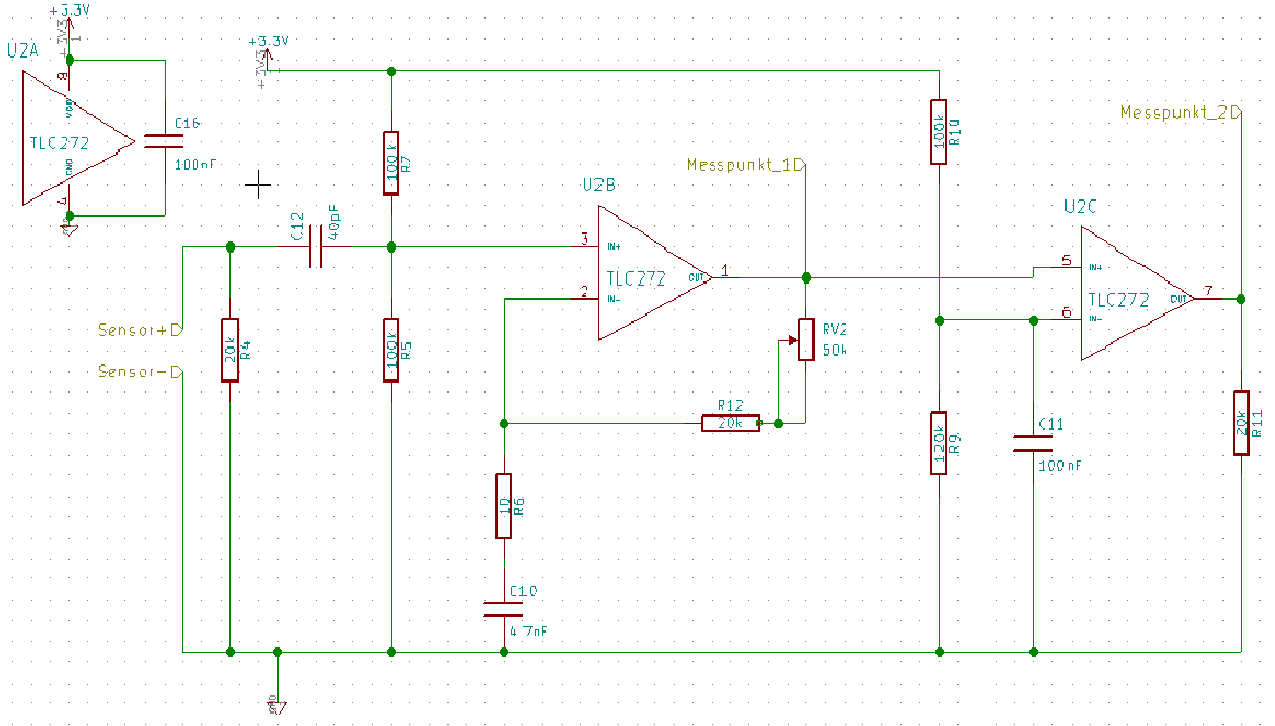
\includegraphics[width=1\textwidth%, draft
]{Abbildungen/Empfaenger.png}
\captionof{figure}{Empfängerschaltung}
\label{fig:Empfaengerschaltung}
\end{minipage}\\
\end{center}
\subsection{Besonderheit der Software}
\label{Besonderheit der Software}
Um die die Lesbarkeit des Programms zu fördern wurden APIs (Application Programming Interface) verwendet die schon das passende Register ansteuern anstatt per Hand aus dem Reference Manuel jedes einzelne Register rauszusuchen. Das erlaubt Programme leichter zuwarten und zu optimieren. Die APIs lassen sich in der XMC Lib finden, dies ist eine Bibilothek die der Hersteller zuverfügung stellt.
Um .mode zu bearbeiten und nach der erforderten Funktion zu konfigurieren reicht es die  \textit {xmc1-gpio.h} zu betrachten. Somit reicht es in das Feld .mode=gewünschte Funktion ein zu eintragen, in diesem Beispiel ist es \textit{XMC GPIO MODE NPUT PULL UP}.
Siehe\ref{fig:API} : Die API für ein Programmbeispiel anhand einer PULL-UP Initialisierung.
\\
\begin{minipage}{1\textwidth}
\begin{lstlisting}
Code vom Infineon Prozessor XMC 1xxx48 mit der API:
void pin_in_pullup_init(XMC_GPIO_PORT_t *const port, const uint8_t pin)
{
  const	XMC_GPIO_CONFIG_t pin_in_config = {
  			.mode             = XMC_GPIO_MODE_INPUT_PULL_UP, /**< Defines the direction and characteristics of a pin */
  			.output_level     = XMC_GPIO_OUTPUT_LEVEL_HIGH, /**< Defines output level of a pin */
  			.input_hysteresis	= XMC_GPIO_INPUT_HYSTERESIS_STANDARD /**< Defines input pad hysteresis of a pin */
  		};

  XMC_GPIO_Init(port, pin, &pin_in_config);
/*
 * Initializes input / output mode settings like, pull up / pull down devices,push pull /open drain, and pad driver mode.
 * Also configures alternate function outputs and clears hardware port control for selected \a port and \a pin .
 * It configures hardware registers Pn_IOCR,Pn_OUT,Pn_OMR,Pn_PDISC and Pn_PDR.\n
*/
}
\end{lstlisting}
\captionof{figure}{Die API für ein Programmbeispiel anhand einer PULL-UP Initialisierung}
\label{fig:API}
\end{minipage}

 In der\ref{fig:oAPI} Teilausschnitt von der GPIO Init in der xmc1 gpio.c Datei, veranschaulicht gut was hinter API passiert. Es erfordert viel Einarbeitung in den Prozessor um die einzelnen Funktionsaufrufe zu verstehen, somit erleichter die API die Programmierarbeit und ist zeitgleich Anwenderfreundlich.


%Pn_OMR=	Pn_OMR | (1<<Port);		//Port Output Modification
%Pn_PDISC=	Pn_PDISC &~ (1<<Port);	//Pin Function Decsision Control Register
%Pn_PDR=	Pn_PDR 	 | (1<<Port);	
\begin{minipage}{1\textwidth}
\begin{lstlisting}
void XMC_GPIO_Init(XMC_GPIO_PORT_t *const port, const uint8_t pin, const XMC_GPIO_CONFIG_t *const config)
{
  XMC_ASSERT("XMC_GPIO_Init: Invalid port", XMC_GPIO_CHECK_PORT(port));
  XMC_ASSERT("XMC_GPIO_Init: Invalid mode", XMC_GPIO_IsModeValid(config->mode));
  XMC_ASSERT("XMC_GPIO_Init: Invalid input hysteresis", XMC_GPIO_CHECK_INPUT_HYSTERESIS(config->input_hysteresis));
  
  /* Switch to input */
  port->IOCR[pin >> 2U] &= ~(uint32_t)((uint32_t)PORT_IOCR_PC_Msk << (PORT_IOCR_PC_Size * (pin & 0x3U)));

  /* HW port control is disabled */
  port->HWSEL &= ~(uint32_t)((uint32_t)PORT_HWSEL_Msk << ((uint32_t)pin << 1U));

  /* Set input hysteresis */
  port->PHCR[(uint32_t)pin >> 3U] &= ~(uint32_t)((uint32_t)PORT_PHCR_Msk << ((uint32_t)PORT_PHCR_Size * ((uint32_t)pin & 0x7U)));
  port->PHCR[(uint32_t)pin >> 3U] |= (uint32_t)config->input_hysteresis << ((uint32_t)PORT_PHCR_Size * ((uint32_t)pin & 0x7U));
.
.
.    
\end{lstlisting}
\captionof{figure}{Teilausschnitt von der GPIO Init in der xmc1 gpio.c Datei }
\label{fig:oAPI}
\end{minipage}

xmc1-gpio.c sowie xmc1-gpio.h lassen sich in der XMC Libary im Anhang finden.

